\section{Design Details}
\label{designdetails}

Some changes were done along the way in order to accomodate new ideas and solve issues that occured. The changes were of differing size and complexity, but we are in the opinion that our original architecture was a good fit for what we wanted to accomplish. 

Our main quality attribute, modifiability, laid some guidelines for the architecture, since we had to consider modifiability at all stages of the development. 

Listed below are the features we wish to highlight.
Each item will be described in detail in the follow subsections.

\begin{itemize}
	\item \textbf{bedpresBingo.BingoCell} 
	\item \textbf{bedpresBingo.BingoView} 
	\item \textbf{bedpresBingo.GameActivity}
	\item \textbf{bedpresBingo.ServerCommunication} 
	\item \textbf{bedpresBingo.MainActivity} 
	\item \textbf{Server} 
\end{itemize}


\subsection{bedpresBingo.BingoCell}
This class is used as a model for the bingo cells in order to ensure that the bingo cells accomodate a common standard. An instance of the class also acts as a model for a bingo cell. 

An instance of the class has methods for knowing if the cell is selected, via the isSelected() method. The toggleSelected() method is used to toggle if the cell is shown as selected or not. The draw() method is used to draw the visual representation of the bingo cell. 

By having this model we make it a lot easier to reuse code when making the bingo board.

\subsection{bedpresBingo.BingoView}
This class is used as a view controller and a creator of the graphical bingo board. The class holds a double array of instances of the BingoCell class, in order to create a square bingo board. The buildBoard() method is used to create the board. 

The BingoView class has methods to work as a controller. The onCellTouchListener() will create listener for each seperate cell in order to act as a controller for the bingo cell. The setGoldenWord() method will set the golden word in order to tell one cell to become a golden cell. 

The BingoView class also has some logic in order to check if the player achieves a bingo. The method hasBingo() will run for-loops checking the BingoCell instances if all in a row or column is selected and if a golden word is a part of the row or column.

The Bingo View class will also act as a controller controlling its own view. This is possible because of the way Android is built. When something interesting occurs, eg. you achieve a bingo, another player achieves bingo or something is wrong, a toast\footnote[1]{Not a toast you can eat, but rather a small textline shown on screen for a short period of timeg}. 


\subsection{bedprisBingo.GameActivity}
Android is built around having activities for seperate screens in the application. Basically when you change screen, you change activity. The GameActivity class instanciates a BingoView and a ServerCommunication in order to create a game. The class itself does very little.


\subsection{bedpresBingo.MainActivity}
The Main Activity is not a very interesting class. It is added to this documentation in order to shine some light on how Android works. When the application starts, the MainActivity is launched. The activity in our project launches two buttons and a menu. The main functionality of the application is implemented in other classes, and this class is more like a ``Welcome screen''. 


\subsection{bedpresBingo.ServerCommunication}
The ServerCommunication takes care of all communication between the server and the client. The singleton pattern is used in order to ensure that only a single instance of this class occurs. More than one class would make a lot of mess in terms of communication. 

The main reason for parting this functionality into a separate class is modifiability and to more easily keep an overview while coding. By parting the code into seperate classes it was also easier to work in parallell. 

The getBoardFromServer() method will ask the server for a board, and hopefully a string of words is returned, which BingoView later will use to build the board. The method also spawns a pollerThread in order to poll the server for updates regarding other players results.

In order to achieve the goals of availability we have implemented methods for keeping score of a players game. When a player disconnects and then connects again, the getGameURIFromServer will return the game to the player, so the player may continue where he/she was before he/she was disconnected.


\subsection{Server}
The server keeps track on the players, the active game, a company owning the game, and all the active boards. When a client starts a new game, it basically asks the server for a board on the current running game. The server then checks if this player previsouly had an active board running on this game. If a board is found, the player will receive its old board. if not it will return a new randomized board.

\begin{itemize}
	\item A game is always assigned to a company
	\item there will only be one game running at any time. 
	\item Every games has a set of terms assigned to it
	\item Every board will receive a random subset of terms from the active game
\end{itemize}

When a player gets a BINGO! It'll notice the server about which kind of bingo it accomplished. The server will then return this information to all other clients when they request the information. Which happens every 3 seconds.

\subsubsection{The system}
The server is written in Python using the Django web framework. Django appears to be a MVC-framework where we mainly will manage the models and the views for data handling and representation. The application will also contain a twist of observer-observable pattern for the client to observe changes on the server.

Inside of django we'll be using a webservice API framework called tastypie. This let us create a REST-style interfaces for our service. With our REST-service the clients only needs to request and send data back and forth with some simple JSON over http.

Each modules of the system is devied into separated apps to easen a later maintenance process, and to easen the development process without cluttering the workspace.

\subsection{Class Diagram}

\begin{center}
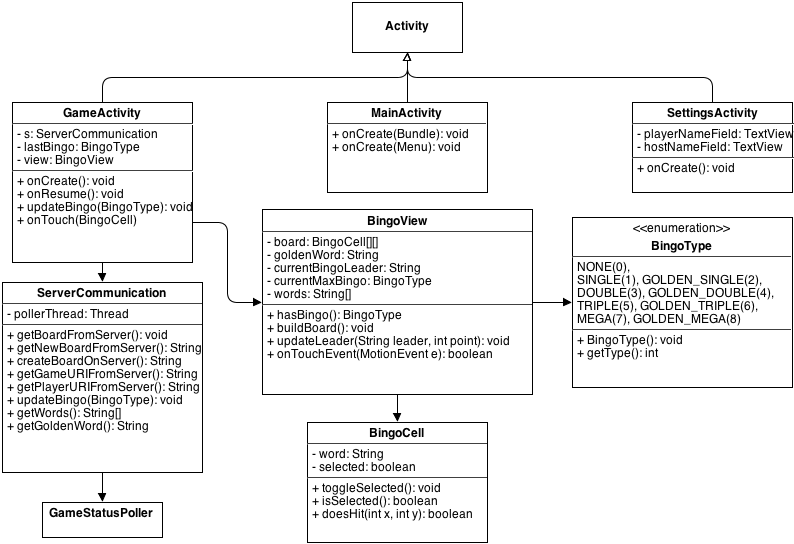
\includegraphics[scale=0.5]{Pikks/ClassDiagramFinal}
\captionof{figure}{Class Diagram for Bedpres Bingo}
\end{center}